\subsection{Unauthenticated Routes}

On all \gls{cpe}s, at least two pages don’t require authentication for their contents to be viewed, the status and about pages. No other pages that can be accessed through the menu seem to work without proper authentication, but it is known that some pages of the web interface are not indexed and can only be accessed directly with their \gls{url}.

It is possible to make some hidden pages visible on \glspl{cpe} 0 and 1 by exporting the configuration file as previously mentioned, changing \texttt{PADRAO\_WIFI\_ONLY} from \texttt{0x0} to \texttt{0x1}, and reimporting the file. But to list all pages available on the \gls{http} Management Interface with certainty, the firmware image of each \gls{cpe} was expanded and inspected. 

To perform this operation, the binwalk tool was used. It takes a binary file and looks for different magic numbers of different file types, detecting which each segment of the file is. Then it is able to extract the individual segments and expand them.

By feeding the firmware images to binwalk, it was verified that \gls{cpe} 5 also carries the management interface of subsidiaries of the \gls{isp} in other countries. A configuration flag indicates which firmware should be used by the \gls{cpe} upon start. As the other management are not accessible without tampering with the device, their files were not inspected.

When testing the different \glspl{url} by using the file names, surprisingly, there was a serious finding on \gls{cpe} 5. The page responsible for importing and exporting configuration files doesn’t require authentication, as shown on Figure \ref{figure:unauthenticated_cpe_configuration_import}. Meaning that anyone that is able to send requests to the port 80/tcp is able to change any setting on the device, including the password of the management console, making null and void any kind of security on the management interfaces of the device.

\begin{figure}[h]
    \centering
    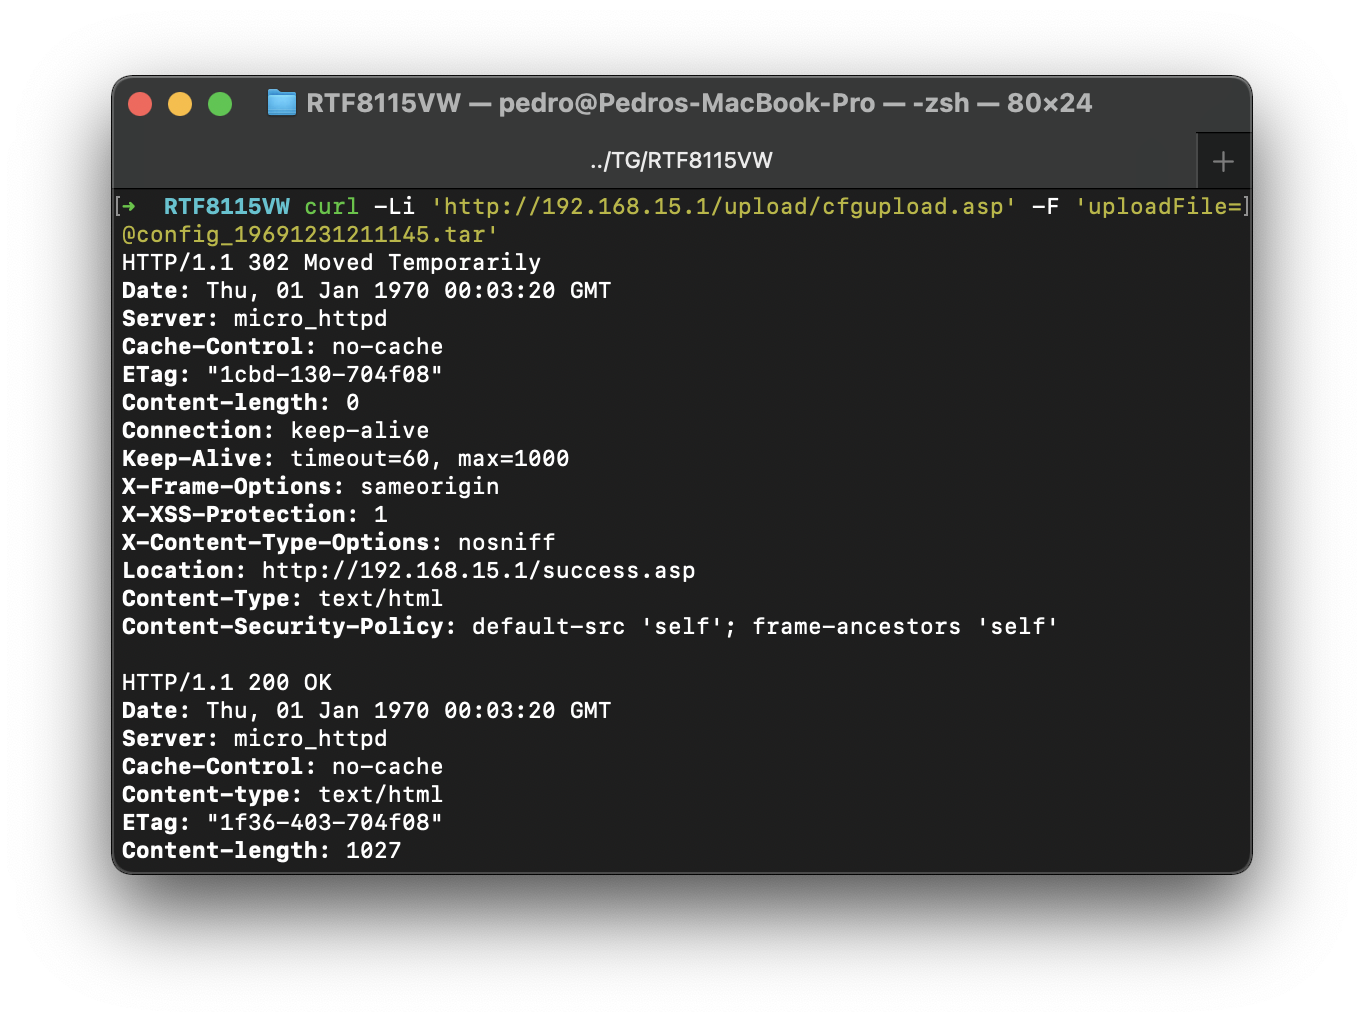
\includegraphics[width=\linewidth]{contents/http-management-interface-analysis/unauthenticated-routes/unauthenticated-cpe-configuration-import.png}
    \caption{Unauthenticated \gls{cwmp} Configuration Import}
    \label{figure:unauthenticated_cpe_configuration_import}
\end{figure}

\FloatBarrier
